\documentclass[10pt,fleqn]{article} % Default font size and left-justified equations
\usepackage[%
    pdftitle={Modélisation SLCI : Stabilité des systèmes},
    pdfauthor={Xavier Pessoles}]{hyperref}
    
\input{style/new_style}
\input{style/macros_SII}
\usepackage{multicol}
\usepackage{siunitx}
%\usepackage{picins}
\fichetrue
%\fichefalse

\proftrue
%\proffalse

\tdtrue
%\tdfalse

\courstrue
\coursfalse

\def\discipline{Sciences \\Industrielles de \\ l'Ingénieur}
\def\xxtete{Sciences Industrielles de l'Ingénieur}

\def\classe{PSI$\star$ -- MP}
\def\xxnumpartie{\textsf{Cycle 02}}
\def\xxpartie{Modéliser les systèmes asservis dans le but de prévoir leur comportement}


\def\xxnumchapitre{Chapitre 1 \vspace{.2cm}}
\def\xxchapitre{\hspace{.12cm} Stabilité des systèmes}


\def\xxtitreexo{Colle 01}
\def\xxsourceexo{\hspace{.2cm}}% \footnotesize{F. Mathurin}}


\def\xxposongletx{2}
\def\xxposonglettext{1.45}
\def\xxposonglety{20}
%\def\xxonglet{Part. 1 -- Ch. 3}
\def\xxonglet{Cycle 02}

\def\xxactivite{Colle 01}
\def\xxauteur{\textsl{X. Pessoles}}

\def\xxcompetences{%
\textsl{%
\textbf{Savoirs et compétences :}\\
%Les sources sont associées par un \emph{hacheur série}. La détermination des grandeurs électriques associées à ce montage permet de conclure vis à vis du cahier des charges.
%\noindent \textbf{Résoudre :} à partir des modèles retenus :
%\begin{itemize}[label=\ding{112},font=\color{ocre}] 
%\item choisir une méthode de résolution analytique, graphique, numérique;
%\item mettre en \oe{}uvre une méthode de résolution.
%\end{itemize}
%\begin{itemize}[label=\ding{112},font=\color{ocre}] 
%\item \textit{Rés -- C1.1 :} Loi entrée sortie géométrique et cinématique -- Fermeture géométrique.
%\end{itemize}
%
%\noindent \textit{Mod2 -- C4.1 :} Représentation par schéma bloc.
}}

\def\xxfigures{
%\includegraphics[width=.6\linewidth]{images/fig_01}
}%figues de la page de garde


\def\xxpied{%
Cycle 02 -- Modéliser les systèmes asservis dans le but de prévoir leur comportement\\
Chapitre 1 -- \xxactivite%
}

\setcounter{secnumdepth}{5}
%---------------------------------------------------------------------------

\usepackage{pgfplots}
\begin{document}

%\chapterimage{png/Fond_Cin}
\input{style/new_pagegarde}
\vspace{8cm}
\pagestyle{fancy}
\thispagestyle{plain}

\def\columnseprulecolor{\color{ocre}}
\setlength{\columnseprule}{0.4pt} 

\def\pathfig{images}

\begin{multicols}{2}
On considère la fonction de transfert en boucle ouverte d’un système :
$G(p)=\dfrac{2}{\left( 10p+1\right)^3}$.

\subparagraph{}\textit{Tracer le schéma-blocs.}

\subparagraph{}\textit{Tracer les diagrammes de bode de $G(p)$.}
\subparagraph{}\textit{Tracer la marge de gain et la marge de phase.}

On place ce système dans une boucle de régulation à retour unitaire en le précédant d’un correcteur proportionnel $C(p)=K$.

%\subparagraph{}\textit{Calculer la valeur de K qui assure la stabilité théorique du système (critère de Routh)}
\subparagraph{}\textit{Calculer la valeur de $K$ de manière à obtenir une marge de phase supérieure ou égale à 45\degres.}
\subparagraph{}\textit{Calculer la valeur de l’écart statique en réponse à un échelon puis en réponse à une rampe.}

On change le correcteur proportionnel, par un correcteur intégral de fonction de transfert $C(p)=\dfrac{Ki}{p}$.

\subparagraph{}\textit{Calculer la nouvelle valeur de l’écart statique en réponse à un échelon puis en réponse à une rampe.}

 
\end{multicols}

\newpage

\subparagraph{}\textit{Identifier la fonction de transfert à partir des diagrammes de bode.}



\begin{center}
\includegraphics[width=.9\linewidth]{images/fig_01}
\end{center}

\begin{center}
\rotatebox{90}{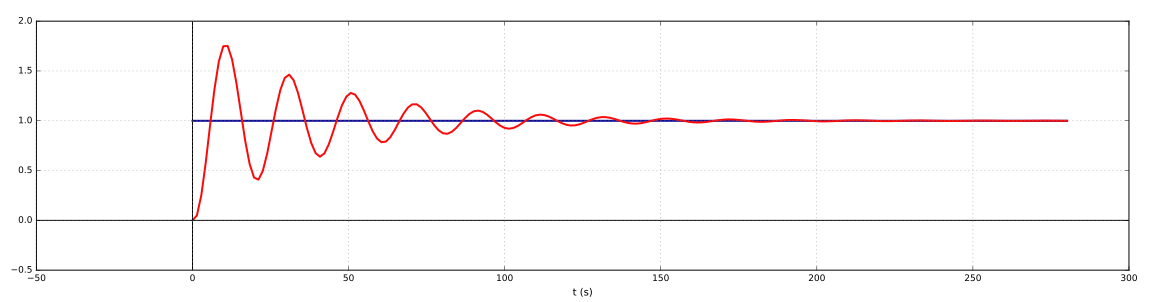
\includegraphics[width=.6\linewidth]{images/fig_02}}
\end{center}



\newpage

\begin{center}
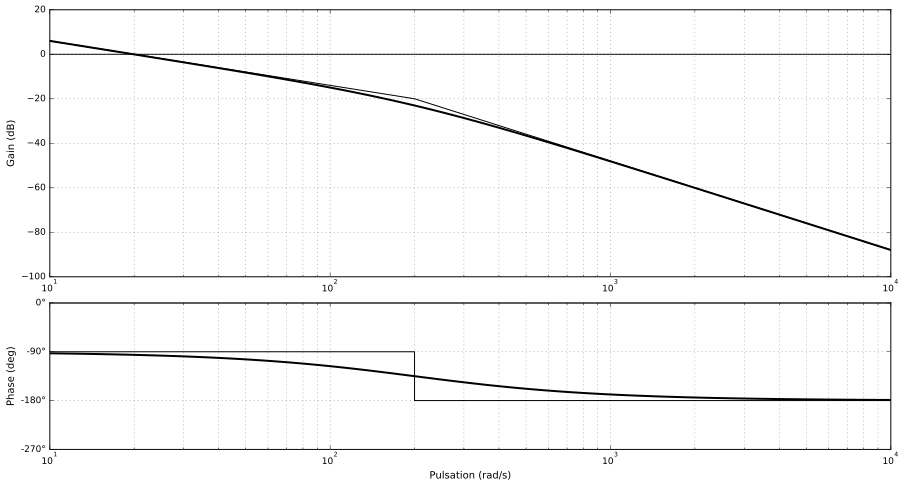
\includegraphics[width=\linewidth]{images/cor_01}

\includegraphics[width=\linewidth]{images/cor_02}

\includegraphics[width=\linewidth]{images/cor_03}

\includegraphics[width=\linewidth]{images/cor_04}
\end{center}

\end{document}


\begin{center}
\includegraphics[width=\linewidth]{images/fig_06}
\end{center}

\begin{center}
\end{center}

\subparagraph{}\textit{}




